\documentclass[11pt]{article}
\usepackage{comment} % enables the use of multi-line comments (\ifx \fi) 
\usepackage{fullpage} % changes the margin
\usepackage{listings}
\usepackage{enumitem}
\usepackage{graphicx}
\graphicspath{ {images/} }

\begin{document}
% Header
\noindent
\large\textbf{Assignment 4} \hfill \textbf{Team 11} \\
\normalsize CSC488 \hfill Faith Magcalas - g3hummus \\
Prof. Wortman \hfill Jingnan Chen - c6chenjl \\
TA: Peter McCormick \hfill Qi Jian Huang - c6huangu \\
\hspace*{0pt} \hfill Steven Low - g3lowste

% -------------------- Global stuff ---------------------
\section*{Global Instructions}
\begin{enumerate}
\item Unconditional branch, where label is the address:
\begin{lstlisting}
    BR label:
        PUSH label
        BR
\end{lstlisting}

\item Conditional branch, where label is the address:
\begin{lstlisting}
    BF label:
        PUSH label
        BF
\end{lstlisting}

\item False expression equals MACHINE\_FALSE yields MACHINE\_TRUE (false = false yields true)
\begin{lstlisting}
    NOT: 
        PUSH MACHINE_FALSE
        EQ
\end{lstlisting}

\end{enumerate}

% --------------------- Storage -------------------------
\section*{Storage}

Lexical level (LL):
\begin{itemize}
\item will start with 0 at main program scope, and will be 
    incremented if new scope is created within current scope.
\end{itemize}
Order number (ON):
\begin{itemize}
\item representing the offset of the identifier from the beginning of the
    activity record, it will be incremented by the size of each added 
    identifier (1 word for integer and boolean scalar variables, and (1 x
    number of elements) words for arrays).
\end{itemize}
Addressing:
\begin{itemize}
    \item scalar variable address within the activation record is 
    calculated based on sum of starting address of the 
    activation record and the order number for the identifier).
    
    \item array variable address within the activation record is
    calculated based on sum of starting address of the
    activation record and the order number for the identifier.
    
    \item the array element is computed by adding row offset and 
    column offset to the starting array address.
    
    \item for 1D array, the row offset is the difference between the
    accessed index and the lower bound for the array (row\_offset =
    accessed\_index - lb\_index).
    
    \item for 2D array, the row offset is the difference between the
    accessed index and the lower bound in first dimension and multiply
    by the length of second dimension array (row\_offset = 
    (accessed\_index (1st D) - lb\_index (1st D) * (2nd dimension array
    length). The column offset is the difference between the accessed
    index and lower bound in second dimension (col\_offset =
    (accessed\_index (2nd D) - lb\_index (2nd D)). 
\end{itemize}

\begin{enumerate}[label=(\alph*)]
\item \textbf{Variables in the main program}\\
In the main program, storage for variables will be allocated in the 
activation record of its containing scope (aka the main program). For
each identifier, its lexical level and order number will be stored 
within the symbol table entry, and all identifiers’ values are 
determined during semantic analysis.\\
\\
Examples:\\
Assume a variable x is defined, first assign integer constant 2
into variable x (x = 2), then perform operation x = x + 3
    \begin{lstlisting}
    ADDR LL ON    // address of variable x on stack
    PUSH 2        // push integer constant 2 onto stack
    STORE         // store integer constant 2 into variable x in memory 
    ADDR LL ON    // address of variable x on stack
    ADDR LL ON    // address of variable x on stack again
    LOAD          // load the value of x from memory address onto stack
    PUSH 3        // push integer constant 3 onto stack
    ADD           // perform addition (3 + x)
    STORE         // store (3 + x) into address of x in memory
    \end{lstlisting}

\item \textbf{Variables in procedures and functions}\\
    Variables in procedures and functions are handled similar to
    variables in main program, except the lexical level will be greater
    than 0.
    
\item \textbf{Variables in minor scopes ( e.g. ’\{’ declaration
              statement ’\}’ )}\\
    Declared identifiers within a minor scope will belong to its major
    scope, which it means the lexical level will be the same, no new
    lexical level is created at this point.
    
\item \textbf{Integer and boolean constants ( e.g. `true' and
              `false' )}\\
    Integer and boolean constants will be pushed onto stack where needed,
    no need to allocate storage space for them.\\
    \\
    Examples:
    \begin{itemize}
    \item integer constant 5: 
    \begin{lstlisting}
    PUSH 5
    \end{lstlisting}
    
    \item boolean constant true: 
    \begin{lstlisting}
    PUSH MACHINE_TRUE
    \end{lstlisting}
    
    \item boolean constant false:
    \begin{lstlisting}
    PUSH MACHINE_FALSE
    \end{lstlisting}
    \end{itemize}
    
\item \textbf{Text constants ( e.g. ``Like This'' )}\\
    Text constants will be pushed onto stack as required.\\
\\
Example:
\begin{itemize}
\item write "cat":
	\begin{lstlisting}
    PUSH "c"
    PRINTC
    PUSH "a"
    PRINTC
    PUSH "t"
    PRINTC
    \end{lstlisting}
\end{itemize}
\end{enumerate}

% -------------------- Expressions ------------------------
\section*{Expressions}
\begin{enumerate}[label=(\alph*)]
\item \textbf{Describe how the values of constants (including text
    constants) will be accessed.}\\
    Push them onto stack as there is no need to store these values in
    the memory. See examples in Storage (d) and (e)
    
\item \textbf{Describe how the values of scalar variables will be
	accessed.}\\
	To access a value of scalar variable, the variable's memory address
    is pushed onto the stack, and then load the value of that memory
    address onto the stack.\\
    \\
    Example:
    \begin{lstlisting}
    ADDR LL ON        // Scalar variable address
    LOAD              // Load the value from address to stack
    \end{lstlisting}
    
\item \textbf{Describe how array elements will be accessed.
Show details of array subscripting in the general case for one and two
dimensional arrays.}\\

    For details, refer to "Storage $\rightarrow$ Addressing" section.\\
    \\
Examples:\\
For 1D:
\begin{itemize}
\item array base address:
	\begin{lstlisting}
    ADDR LL ON
    \end{lstlisting}

\item calculate row offset
    \begin{lstlisting}
    PUSH accessed_index
    PUSH lb_index
    SUB
    \end{lstlisting}
\item add the offset to the array base address
    \begin{lstlisting}
    ADD
    \end{lstlisting}
\item load the value of the address onto stack
    \begin{lstlisting}
    LOAD
    \end{lstlisting}
\end{itemize}
For 2D:
\begin{itemize}
\item array base address:
	\begin{lstlisting}
    ADDR LL ON
    \end{lstlisting}
\item calculate the row offset
	\begin{lstlisting}
    PUSH accessed_index_1D
    PUSH lb_index_1D
    SUB
    PUSH array_length_2D
    MUL
    \end{lstlisting}
\item calculate the col offset
	\begin{lstlisting}
    PUSH accessed_index_2D
    PUSH lb_index_2D
    SUB
    \end{lstlisting}
\item add row and col offset then add it to array base address
	\begin{lstlisting}
    ADD
    ADD
    \end{lstlisting}
\item load the value of the address onto stack
	\begin{lstlisting}
    LOAD
    \end{lstlisting}
\end{itemize}

\item \textbf{Describe how you will implement each of the arithmetic operators +, -, *, and /}\\
    Arithmetic operators are already implemented in the machine
    instructions (ADD, SUB, MUL, DIV, NEG). They are implemented by
    recursively evaluating the two operands and then use the provided
    instruction to compute the operator result from the two evaluated
    operands.\\
\\
Examples:
\begin{itemize}
\item 1 + 2:
\begin{lstlisting}
    PUSH 1
    PUSH 2
    ADD
\end{lstlisting}
\item 2 - 1:
\begin{lstlisting}
    PUSH 2
    PUSH 1
    SUB
\end{lstlisting}
\item 2 * 1:
\begin{lstlisting}
    PUSH 2
    PUSH 1
    MUL
\end{lstlisting}
\item 2 / 1:
\begin{lstlisting}
    PUSH 2
    PUSH 1
    DIV
\end{lstlisting}
\item -5:
\begin{lstlisting}
    PUSH 5
    NEG
\end{lstlisting}
\end{itemize}

\item \textbf{Describe how you will implement each of the comparison
    operators $<$ , $<=$, $=$, `not$=$', $>=$, $>$.}\\
The operators "LT" and "EQ" is provided, the other operators will be
transformed using provided operators.\\
\\
Examples:
\begin{itemize}
\item 1 $<$ 2:
\begin{lstlisting}
    PUSH 1
    PUSH 2
    LT
\end{lstlisting}
\item 2 $<=$ 3: same as 3 not $<$ 2
\begin{lstlisting}
    PUSH 2
    PUSH 3
    SWAP
    LT
    NOT
\end{lstlisting}
\item 2 $=$ 2:
\begin{lstlisting}
    PUSH 2
    PUSH 2
    EQ
\end{lstlisting}
\item 3 not$=$ 2:
\begin{lstlisting}
    PUSH 3
    PUSH 2
    EQ
    NOT
\end{lstlisting}
\item 3 $>=$ 2: same as 3 not $<$ 2
\begin{lstlisting}
    PUSH 3
    PUSH 2
    LT
    NOT
\end{lstlisting}
\item 3 $>$ 2: same as 2 $<$ 3
\begin{lstlisting}
    PUSH 3
    PUSH 2
    SWAP
    LT
\end{lstlisting}
\end{itemize}

\item \textbf{Describe how you will implement each of the boolean operators `and' , `or' , `not'}\\
Although there is a machine instruction `OR', we will not be able to use it as it won't properly short circuit the operators, so instead we will handle or/and as follows:
\begin{itemize}
\item `x or y': First we evaluate x and then check if we \textbf{cannot} short circuit, in which case we BF to \_next. If we can short circuit however, we push the MACHINE\_TRUE that was absorbed by BF back onto the stack, and then branch to \_end.\\
\\
Or example:
\begin{lstlisting}
    emit code to evaluate x
    BF _next
    PUSH MACHINE_TRUE
    BR _end
    _next:
        emit code to evaluate y
    _end:
        // ending code i.e. store, etc
\end{lstlisting}
\item `x and y': First we evaluate x and then check if we \textbf{can} short circuit, in which case we BF to \_false where we PUSH MACHINE\_FALSE. If we cannot short circuit however, we evaluate y and then branch to \_end.\\
\\
And example:
\begin{lstlisting}
    emit code to evaluate x
    BF _false
    emit code to evaluate y
    BR _end
    _false:
    	PUSH MACHINE_FALSE
    _end:
    	// ending code i.e. store, etc
\end{lstlisting}

\item `not x':
\begin{lstlisting}
    emit code to evaluate x
    NOT
\end{lstlisting}
\end{itemize}

\item \textbf{describe how you will implement conditional
	expressions}\\
conditional expressions are implemented using comparison operators 
and conditional/unconditional branch. In below examples, conditional
statements also included.\\
\\
Example: bool $=$ (3 $<$ 5 ? true : false): 
assume boolean scalar variable "bool" is defined
\begin{lstlisting}
    ADDR LL ON        \\ 'bool' variable address
    PUSH 3            
    PUSH 5
    LT                \\ compare using 'LT' comparator
    BF _label_else    
    PUSH MACHINE_TRUE
    BR _label_end
    _label_else:
        PUSH MACHINE_FALSE
    _label_end:
        STORE         \\ store result into 'bool'
\end{lstlisting}

\end{enumerate}

% ----------------- Functions and Procedures ------------------
\section*{Functions and Procedures}
\begin{enumerate}[label=(\alph*)]
\item \textbf{Activation record for functions and procedures}\\
\begin{center}
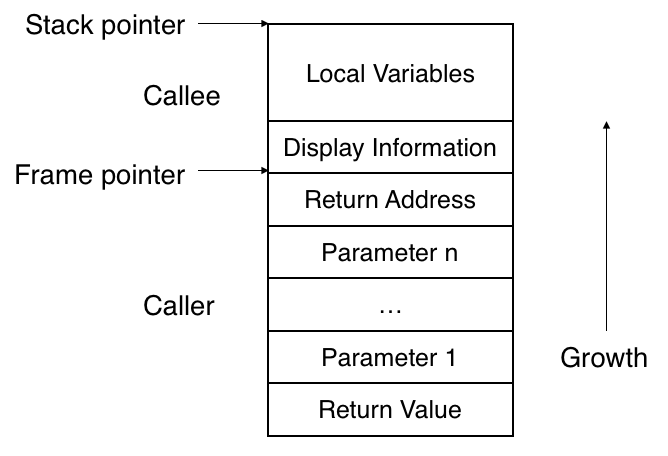
\includegraphics[scale=0.75]{activation_record}
\end{center}

\item \textbf{Procedure and function entrance code}\\
When entering a routine (procedure or function) both the caller and callee have different responsibilities for setting up the activation record. The caller of a function is responsible for pushing a space for the return value, as well as the parameters and return address, however, a procedure call does not need to have a space for return value. The caller then branches to the callee, who takes care of display management and pushes the local variables onto the stack. A generic example is shown below\\
Example:
\begin{itemize}
\item Caller responsibilities:
\begin{lstlisting}
    PUSH UNDEFINED              // return value.
    PUSH parameter_1
    ...
    PUSH parameter_n
    PUSH program_counter        // return address
    BR callee_address           // branch to the callee
\end{lstlisting}
\item Callee responsibilities
\begin{lstlisting}
    ADDR LL 0                   // save the display
    PUSHMT
    SETD LL
    PUSH local_1
    ...
    PUSH local_n
\end{lstlisting}
\end{itemize}

\item \textbf{Procedure and function exit code}\\
Function exit code is responsible for doing essentially the opposite of the
entrance code. First, the callee will push the number of local variables onto
the stack (which we will keep track of,) such that we can use the POPN
instruction to pop them all off the stack, we then restore the display and
branch to the return address. Once there, the caller will do the same POPN
instruction to pop the parameters off the stack, and we will leave the return
value on the stack so the caller can use it. A generic example is shown
below.\\
Example:
\begin{itemize}
\item Callee responsibilities
\begin{lstlisting}
    PUSH n                      // Where n is number of locals
    POPN
    SETD LL
    BR
\end{lstlisting}
\item Caller responsibilities
\begin{lstlisting}
    PUSH n                     // where n is number of parameters
    POPN
\end{lstlisting}
\end{itemize}

\item \textbf{Describe how you will implement parameter
passing}\\
Parameter passing is shown above in function entrance code (part b). The only other consideration not mentioned, is that since a parameter is an expression, we cannot directly push it onto the stack, the expression must first be evaluated before it can be pushed onto the stack. Specific details on expression evaluation can be found in the expression section.\\
Example:
\begin{lstlisting}
    emit code to evaluate parameter_1
    PUSH parameter_1
    ...
    emit code to evaluate parameter_2
    PUSH parameter_2
\end{lstlisting}

\item \textbf{Describe how you will implement function call
and function value return}\\
Function call implementation is described in detail in entrance and exit code
(parts (b) and (c).) The return value of a function is left on top of the stack
when we exit the function, so that it can be used by the callee.

\item \textbf{Describe how you will implement procedure call}\\
Procedure call implementation is described in detail in entrance code and exit
code (parts (b) and (c).) The only difference from procedure to function is
that we do not leave space for return values.

\item \textbf{Describe your display management strategy}\\
Display management is described in function exit and entrance code (part (b)
and (c).) When entering the function, the callee saves the display, and when
exiting the function, the callee restores it.
\end{enumerate}

% ----------------------- Statements -------------------------

\section*{Statements}
\begin{enumerate}[label=(\alph*)]
\item \textbf{Assignment statement}\\
variable := expression
\begin{lstlisting}
    ADDR LL ON
    emit code to evaluate expression
    STORE
\end{lstlisting}

\item \textbf{If statements}\\
'if' expression 'then' statement1 'else' statement2
\begin{lstlisting}
    emit code to evaluate expression
    BF _else
    emit code to execute statement1
    BR _end
    _else:
    	emit code to execute statement2
    _end:
    	// ending code
\end{lstlisting}
'if' expression 'then' statement
\begin{lstlisting}
    emit code to evaluate expression
    BF _end
    emit code to execute statement
    _end:
    	// ending code
\end{lstlisting}

\item \textbf{While and repeat statements}\\
'while' expression 'do' statement
\begin{lstlisting}
    _start:
        emit code to evaluate expression
        BF _end
        emit code to execute statement
        BR _start
    _end:
    	// ending code
\end{lstlisting}
'repeat' statement 'until' expression
\begin{lstlisting}
    _start:
        emit code to execute statement
        emit code to evaluate expression
        BF _start
    // continue when expression true
\end{lstlisting}

\item \textbf{All forms of exit statements}
\begin{itemize}
\item case 1: exit:
    When an exit statement is found, an unconditional branch is
    executed to exit its containing loop.
    
\item case 2: exit integer:
    When an ``exit integer'' is found, an unconditional branch is executed, however
    the exit statement label needs to be the correct loop ending.
    
\item case 3: exit when true:
	The only difference between the previous two is that "exit when true" is using 
    conditional branch "BF" rather than unconditional branch "BR"
    
\item case 4: exit integer when true:
	This case is the combination of case 2 and 3
\end{itemize}

\item \textbf{Return statements}
\begin{itemize}
\item For Procedures:
return statements are not necessary in this case. Usually at the end of a procedure, it should clean up of all the local variables of the procedure on the stack, and also there is an instruction that always branches back to where it gets called and continue  to execute the next instruction.
\item For Functions: return statements are necessary in this case. Usually at the end of a function, we should store the return value to the location that is reversed by the caller, then we clean up of all the local variables of the function on the stack,and also there is an instruction that always branches back to where the function gets called and continue to execute the next instruction.\\
\\
Example:
\begin{lstlisting}
    emit code to find out the reserved address for return value
    ADDR LL -n     // we are tracing back on the stack, and the
                   // offset -n depends on the number of arguments
    SWAP
    STORE
    BR             // Branch back to where the function gets called
                   // (similar in procedure case)
\end{lstlisting}
\end{itemize}
\item \textbf{`read' and `write' statements}
\begin{itemize}
\item 'write' expression
\begin{lstlisting}
    emit code to evaluate expression
    PRINTI
\end{lstlisting}
\item 'write' text\\
for each character:
\begin{lstlisting}
    PUSH character
    PRINTC
\end{lstlisting}
\item 'write' 'newline'
\begin{lstlisting}
    PUSH '\n'
    PRINTC
\end{lstlisting}
\item 'write' sequence of outputs\\
for each output:
\begin{lstlisting}
    check if it's an expression, text, or 'newline'
    emit code to execute appropriate 'write' instructions
\end{lstlisting}
\item 'read' variable
\begin{lstlisting}
    ADDR LL ON
    READI
    STORE
\end{lstlisting}
\item 'read' sequence of variables\\
for each variable:
\begin{lstlisting}
    execute instructions for 'read' variable
\end{lstlisting}
\end{itemize}

\item \textbf{Handling of minor scopes}\\
Statements in minor scopes are treated the same as statements in a major scope.

\end{enumerate}

% ----------------------- Other ------------------------------
\section*{Other}
\begin{enumerate}[label=(\alph*)]
\item \textbf{Main program initialization and termination}\\
A few steps will be done for the main program initialization,
while the termination is done using the machine instruction HALT.\\
\\
Main program initialization:
\begin{itemize}
\item push stack pointer onto stack
\begin{lstlisting}
    PUSHMT 
\end{lstlisting}
\item setup display entry from stack, LL = 0 for main program
\begin{lstlisting}
    SETD LL
\end{lstlisting}
\item reserve enough storage needed for the scope
\begin{lstlisting}
    PUSH UNDEFINED
    PUSH scope_size_in_word
    DUPN
\end{lstlisting}
\end{itemize}
Main program termination:
\begin{lstlisting}
    HALT
\end{lstlisting}

\item \textbf{Any handling of scopes not described above}\\
There is no further handling of scopes needed. The minor scope's
storage requirement is already handled when the major scope is
initialized. The handling of major scopes already is explained in the Storage section.

\item \textbf{Any other information that you think is relevant}\\
The PUSH operations above can be replaced with any other sequence of
operations that result in an integer, a text constant or a boolean
onto the stack where applicable.
\end{enumerate}

\end{document}
